\documentclass[twocolumn]{article}

\usepackage{a4,harvard,graphicx}

% define the vamps logo (think of a nice one!)
\newcommand{\vamps}{{\sf Vamps}}

% the S-Lang logo
\newcommand{\slang}{{\bf S-Lang}}

% Make index stuff a bit easier
\newcommand{\Index}[1]{#1\index{#1}}

%How to print an URL
\newcommand{\url}[1]{#1}
% Some common names etc
\newcommand{\unix}{{\sc unix}}
\newcommand{\ascii}{{\sc ascii}}
\newcommand{\ansi}{{\sc ansi}}
\newcommand{\linux}{Linux}
\newcommand{\netbsd}{Net-{\sc bsd}}
\newcommand{\msdos}{{\sc ms-dos}}
\newcommand{\ostwo} {{\sc OS/2}}
\newcommand{\aix}{{\sc aix}}
\newcommand{\gnu}{{\sc gnu}}
\newcommand{\sunos}{Sun-{\sc os}}

\title{\vamps, a Vegetation-AtMosphere-Plant-Soil water model}
\author{J. Schellekens
\thanks{Vrije Universiteit Amsterdam, The Netherlands; International
Institute for Tropical Forestry, Rio Piedras, Puerto Rico}\\ 
{\tt schj@geo.vu.nl}}
\date{April, 11 1997}

\begin{document}
\setlength{\parindent}{0pt}
\setlength{\parskip}{0.3cm}
\setlength{\textwidth}{1.2\textwidth}

\bibliographystyle{dcu}
\maketitle

\section*{Introduction}
\vamps\ is a one-dimensional water balance model for soils covered
by forest, agricultural crop or bare land particularly suited for use
in tropical environments.  \vamps\ can be used as a complete forest
hydrological model or as a tool to determine just one or more parameters
(e.g. calculate interception using Gash' model). \vamps\ was designed to
be extensible. At the same time the model should be simple to operate. The
model is therefore build in a modular fashion and is equipped with
a simple C-like scripting language.  Features such as  variable time
steps and the ability to select modules allow the model to be used in
both data-rich and data-poor environments. Interactive graphics functions
(on selected operating systems) allow quick visualization of variables
for evaluation of model runs.

The model has been developed as part of a collaborative project
'Hydrological modeling in a humid tropical island setting: with
special reference to The Luquillo experimental Forest, Puerto Rico'
between the International Institute of Tropical Forestry and the Vrije
Universiteit Amsterdam \cite{bruijnzeel1994}.  The model is free and
distributed with complete source code. It runs on a variety of operating
systems\footnote{At the moment \vamps{} runs on several operating
systems including \unix\ (\sunos{}, \linux{}, \netbsd\ and \aix{})
\msdos\ and \ostwo{}}.

The soil part of \vamps{} was developed
after {\sc swatr}\footnote{Currently the swap/swatr program is
maintained and documented in by: Dept. of Agrohydrology, Winand Staring
Centre and Dept. of Water Resources, Wageningen Agricultural
University} \cite{feddes1978273}.  
\begin{table*}[t]
\centerline{
\fbox{\parbox{12cm}{
\begin{itemize}
\item The program is written in \ansi{} C \cite{kernighan1988}
\item Documentation for both model principles and model operation
\item Both binaries and source code available via the World Wide Web
\item Most parts of the model can be used separately
\item Variable time-steps ( e.g. 0.5 seconds to two weeks )
\item No limit to the number of soil layers 
\item Run with \sunos{}, \linux{}, \aix{}, \netbsd{}, \msdos\ and \ostwo
\item Includes pre- and postprocessors
\item Simple \ascii\ input and output file format
\item Easy extension by the users through builtin (high level) library
\item Screen and hardcopy graphics on several platforms
\item Simple to adjust to specific needs at source 
code level
\end{itemize}
}}}
\label{tab:features}
\caption{Selected features of the \vamps\ model}
\end{table*}
The large number of models that have been developed is an indication that
models need to be tailored or adapted for each specific application.
In order to make \vamps\ easily extensible a C-like interpreted
language \cite{davis1995282,davis1995283} allows the user to redefine
builtin functions with functions tailored to the site in question.
These features in combination with testing on several tropical sites make
the model of particular importance to those interested in the tropics
as a whole and tropical forests in particular.

The main development goals of \vamps\ are: {\em (i)} make a parameterized
model which can adequately describe the flow of water in a forested
environment (on a plot base) and {\em (ii)} be flexible enough to be
applied to the variety of forested environments that exist.  Due to
its flexibility it is also possible to apply \vamps\ to plots
covered with agricultural crops or bare soils.  Furthermore the software
is distributed with complete source code and documentation to allow the
user to adapt the program to new situations and examine the program's
internal operation.


\section*{Model principles}
The flow of water through a forested ecosystem is shown in
Figure~\ref{fig:fcycle}. Three pathways are generally 
distinguished by which precipitation reaches the forest floor. A small
fraction of the precipitation reaches the forest floor without touching leaves
or stems. This is known as direct throughfall. Another small 
fraction flows down the tree trunks as stemflow. The remaining fraction
hits the forest canopy and will leave the canopy as
crown drip or evaporate from the wet canopy depending on canopy
storage capacity and shape, the kinetic energy of the droplets and the
atmosphere's evaporative demand.  Water infiltrating the soil
profile can runoff laterally as saturated or unsaturated flow,
percolate to deep groundwater or is extracted by the roots of
plants or trees. If the troughfall intensity exceeds the infiltration
capacity of the topsoil, Hortonian overland flow can occur. The top
layer of the soil profile can become saturated resulting in saturation
overland flow. \vamps\ simulates most of these fluxes which is
illustrated in
\begin{figure}
\centerline{\includegraphics{psfig/fcycle.eps}}
\caption{Simplified diagram of the flow of water through a forested
ecosystem (after \protect\citeasnoun{bruijnzeel1983T})}
\label{fig:fcycle}
\end{figure}
Figure~\ref{fig:vflow}.
The model is mainly driven by input from
the atmosphere\footnote{As the bottom boundary conditions can also
change in time one could probably regard this as a driving force as
well}.
\begin{figure}
\centerline{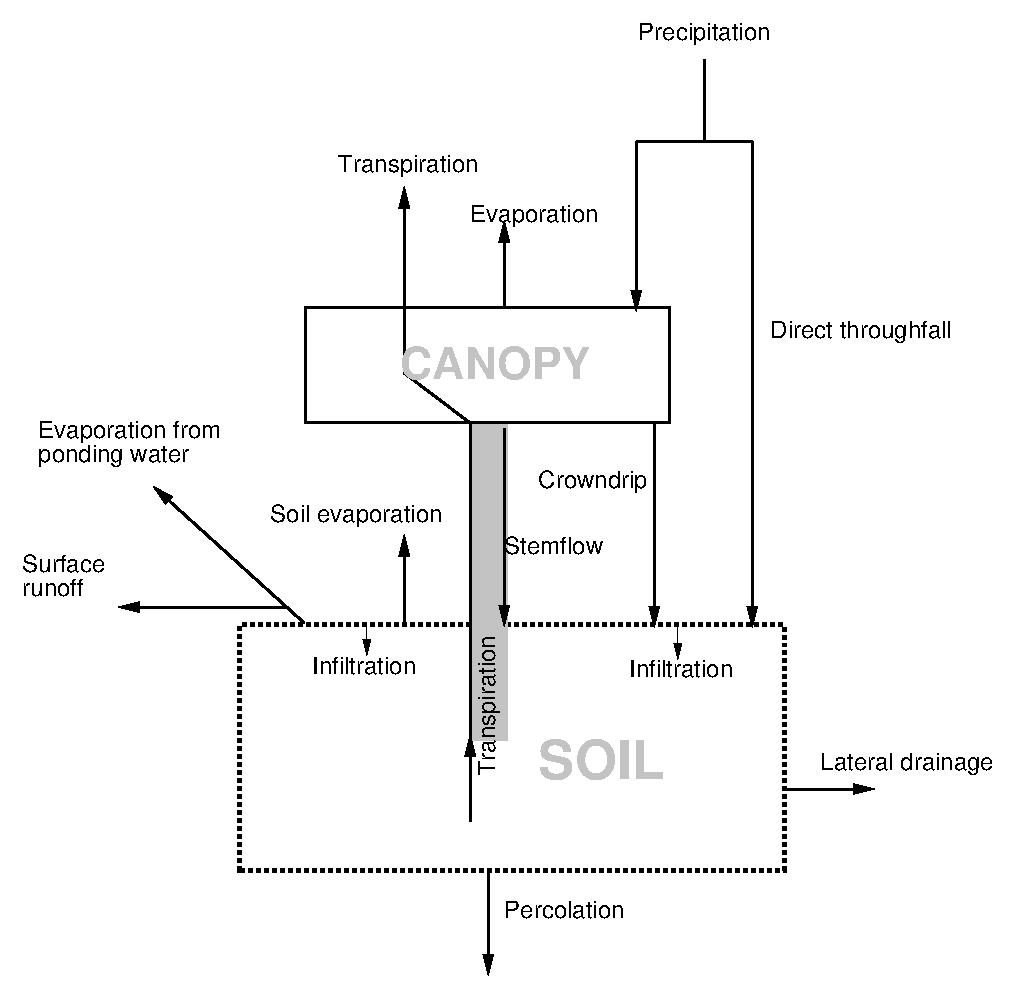
\includegraphics{psfig/vflow.eps}}
\caption{Simplified flow diagram of the \vamps\ model}
\label{fig:vflow}
\end{figure}

Most of the fluxes in the model can either be
calculated or given by the user. The atmosphere, canopy and soil part
of the model can be combined or used separately. However, the strength
of the model is the ability to combine  these parts into an
integrated model for the forest hydrological cycle. 

The following briefly summarizes the methods used to
calculate the water fluxes:
\begin{description}
\item[Throughfall] can be determined in several ways. {\em (1)} using 
a complete canopy water balance model based on the model developed by
 \citeasnoun{rutter1971174}. {\em (2)} using one of the simpler 
analytical approaches by  \citeasnoun{gash1979165} or
 \citeasnoun{calder1986171}.  {\em (3)} the Leaf Area Index based
solution also used by the TOPOG model \cite{vertessy1993140}.

\item[Transpiration] is commonly determined using the Penman-Monteith
equation \cite{monteith1965}. Several alternative methods can be used 
as well \cite{penman1956N,makkink1957,makkink1961,commissie1988N}.

\item[Soil water fluxes] in the unsaturated zone are determined using
Richard's equation. An adapted form of the numerical solution described
by   \citeasnoun{feddes1978273} and  \citeasnoun{belmans1983272} is used.
The relation between water content and pressure head can be
described in several ways 
\cite{genuchten1980179,mualem1976261,clapp1978263}.

\end{description}
These fluxes can also be calculated by a user supplied method.

\section*{Other information}

The latest version and other information is  available on the
\Index{Word Wide Web}
(\url{http://flow.geo.vu.nl}). 

\bibliography{/home/schj/bibtex/artall}
\end{document}

